\documentclass{beamer}
\usepackage[utf8]{inputenc}
\usepackage[T1]{fontenc}
\usepackage[french]{babel}
\usetheme{Hannover}
\usecolortheme{crane}
\usefonttheme{serif}
\usepackage{listings}
\usepackage{multicol}
\usepackage{fixltx2e}


\definecolor{mygreen}{rgb}{0,0.6,0}
\definecolor{myorange}{rgb}{1.0,0.6,0.0}
\definecolor{mygray}{rgb}{0.5,0.5,0.5}
\definecolor{mymauve}{rgb}{0.58,0,0.82}
\lstset{%
  identifierstyle=\color{myorange},
  backgroundcolor=\color{white},   % choose the background color; you must add \usepackage{color} or \usepackage{xcolor}
  basicstyle=\scriptsize,        % the size of the fonts that are used for the code
  breakatwhitespace=false,         % sets if automatic breaks should only happen at whitespace
  breaklines=true,                 % sets automatic line breaking
  captionpos=b,                    % sets the caption-position to bottom
  commentstyle=\color{mygreen},    % comment style
  extendedchars=true,              % lets you use non-ASCII characters; for 8-bits encodings only, does not work with UTF-8
  frame=single,                    % adds a frame around the code
  keepspaces=true,                 % keeps spaces in text, useful for keeping indentation of code (possibly needs columns=flexible)
  keywordstyle=\color{blue},       % keyword style
  morekeywords={}, % if you want to add more keywords to the set
  numbers=left,                    % where to put the line-numbers; possible values are (none, left, right)
  numbersep=5pt,                   % how far the line-numbers are from the code
  numberstyle=\tiny\color{mygray}, % the style that is used for the line-numbers
  rulecolor=\color{black},         % if not set, the frame-color may be changed on line-breaks within not-black text (e.g. comments (green here))
  showspaces=false,                % show spaces everywhere adding particular underscores; it overrides 'showstringspaces'
  showstringspaces=false,          % underline spaces within strings only
  showtabs=false,                  % show tabs within strings adding particular underscores
  stepnumber=1,                    % the step between two line-numbers. If it's 1, each line will be numbered
  stringstyle=\color{mymauve},     % string literal style
  tabsize=2,                       % sets default tabsize to 2 spaces
  title=\lstname                   % show the filename of files included with \lstinputlisting; also try caption instead of title
}

\AtBeginSubsection[]{%
\begin{frame}<beamer>{Table of Contents}
  \begin{multicols}{2}
\tableofcontents[currentsection,currentsubsection,
    hideothersubsections,
    sectionstyle=show/shaded,
    subsectionstyle=show/shaded,
]
  \end{multicols}
\end{frame}
}

\begin{document}

\title{GNU Bison}
\author{Theophile Ranquet
Valentin Tolmer}
\institute{%
  Ecole Pour l'Informatique et les Techniques Avancées\\
  \texttt{ranquet@lrde.epita.fr}\\
  \texttt{nitnelave1@gmail.com}
}

\date{December 17, 2013}

\begin{frame}[plain]
  \titlepage
\end{frame}

\section{Parsers}

\subsection{Grammars and parsers}

\begin{frame}
  \frametitle{What is a parser?}
  \textbf{Parsing}, or \textbf{syntactic analysis} is the process of analysing
  a string of symbols, either in natural language or in computer languages,
  according to the rules of a formal grammar.

  \vfill

  A parser is a software component that takes \textbf{input} data (frequently
  text) and builds a data structure – often some kind of parse tree, abstract
  syntax tree or other hierarchical structure, \textbf{checking} for correct
  syntax in the process.

\end{frame}
\begin{frame}
  The parser is often preceded by a separate \textbf{lexical analyser}, which
  creates tokens from the sequence of input characters; alternatively, these
  can be combined in scannerless parsing.

  \vfill

  Parsers may be programmed by hand or may be automatically or
  semi-automatically generated by a parser generator.

  \vfill

  Parsing is complementary to \textit{templating}, which produces formatted output.
  These may be applied to different domains, but often appear together, such as
  the \texttt{scanf/printf} pair, or the input (front end parsing) and output
  (back end code generation) stages of a \textbf{compiler}.
\end{frame}

\begin{frame}
  \frametitle{Parsing and lexing}
  \begin{center}
    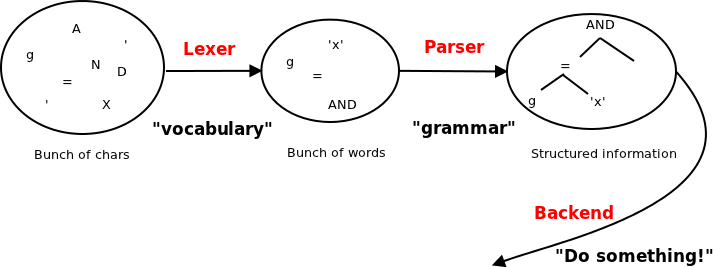
\includegraphics[scale=0.4]{lexer_parser}
  \end{center}
\end{frame}

\begin{frame}
  \frametitle{Grammars and types of parsers}

  An important class of simple parsing is done using \textbf{regular
  expressions}, where a regular expression defines a \textbf{regular language},
  and then the regular expression engine automatically generates a parser for
  that language, allowing pattern matching and extraction of text. In other
  contexts regular expressions are instead used prior to parsing, as the
  \textbf{lexing} step whose output is then used by the parser.

  \vfill

  Programming languages tend to be specified in terms of a deterministic
  context-free grammar because fast and efficient parsers can be written for
  them.
\end{frame}

\begin{frame}
  \frametitle{Context-sensitivity}

  \textbf{Context-free grammars} are limited in the extent to which they can
  express all of the requirements of a language, because they have limited
  \textit{memory}: for example, if a name must be declared before it may be
  referenced.

  \vfill

  Thus, it is a common strategy to create a relaxed parser for a context-free
  grammar which accepts a superset of the desired language constructs (that is,
  it accepts some invalid constructs); later, the unwanted constructs can be
  filtered out at the \textbf{semantic analysis} (contextual analysis) step.
\end{frame}

\begin{frame}[fragile]
  For example, in \textbf{Python} the following is \textit{syntactically} valid
  code:

  \begin{lstlisting}[language=python]
  x = 1
  print x \end{lstlisting}

  The following code, however, is syntactically valid in terms of the
  \textbf{context-free} grammar, yielding a syntax tree with the same structure
  as the previous, but is syntactically \textit{invalid} in terms of the
  \textbf{context-sensitive} grammar, which requires that variables be
  initialized before use:

  \begin{lstlisting}[language=python]
  x = 1
  print y \end{lstlisting}

  Rather than being analyzed at the parsing stage, this is caught by checking
  the values in the syntax tree, hence as part of \textbf{semantic analysis}:
  context-sensitive syntax is in practice often more easily analyzed as
  semantics.
\end{frame}

\begin{frame}
  \frametitle{Compiler design}
  \begin{center}
    %FIXME
    %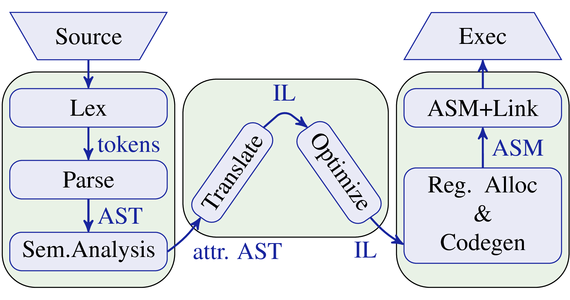
\includegraphics[scale=0.5]{compiler}
  \end{center}
\end{frame}

\begin{frame}
  \frametitle{Types of parsers}
There are (essentially) two ways to parse:
\begin{itemize}
  \item \textbf{Top-down} parsing can be viewed as an attempt to find left-most
derivations of an input-stream by searching for parse trees using a top-down
expansion of the given formal grammar rules. Tokens are consumed from left to
right. \textbf{LL} (\textbf{L}eft-to-Right, \textbf{L}eftmost derivation)
parsers are an example of such parsers.

  \item \textbf{Bottom-up} (or \textit{Shift/Reduce}) parsing starts with the
input and attempts to rewrite it to the start symbol.  Intuitively, the parser
attempts to locate the most basic elements, then the elements containing these,
and so on. \textbf{LR} (\textbf{L}eft-to-right, \textbf{R}ightmost derivation)
parsers are examples of bottom-up parsers.
\end{itemize}
\end{frame}

\begin{frame}
  \frametitle{LL vs LR}
  \begin{center}
    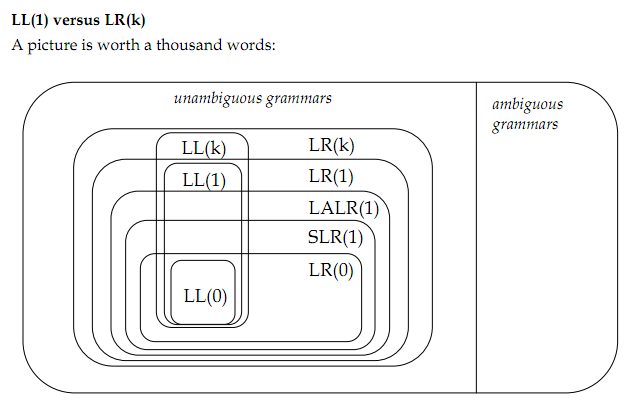
\includegraphics[scale=0.47]{LLLR}
  \end{center}
\end{frame}

\begin{frame}
  \frametitle{Top-down vs bottom-up}
  \begin{center}
    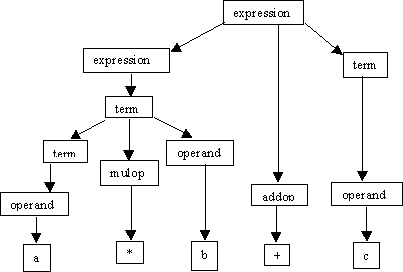
\includegraphics[scale=0.3]{topdown}
\hfill
    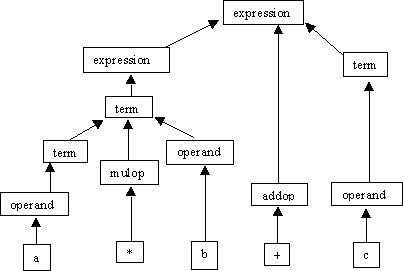
\includegraphics[scale=0.3]{bottomup}
  \end{center}
\end{frame}

\begin{frame}
  \frametitle{Top-down parsing}
  \begin{center}
    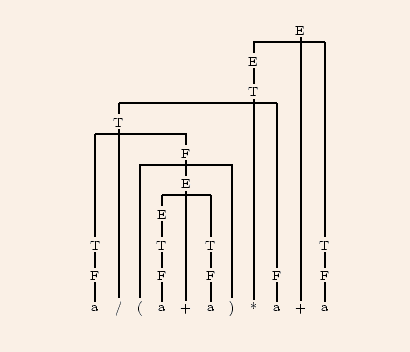
\includegraphics[scale=0.3]{topdown2}
  \end{center}
\end{frame}

\begin{frame}
  \frametitle{Bottom-up parsing}
  \begin{center}
    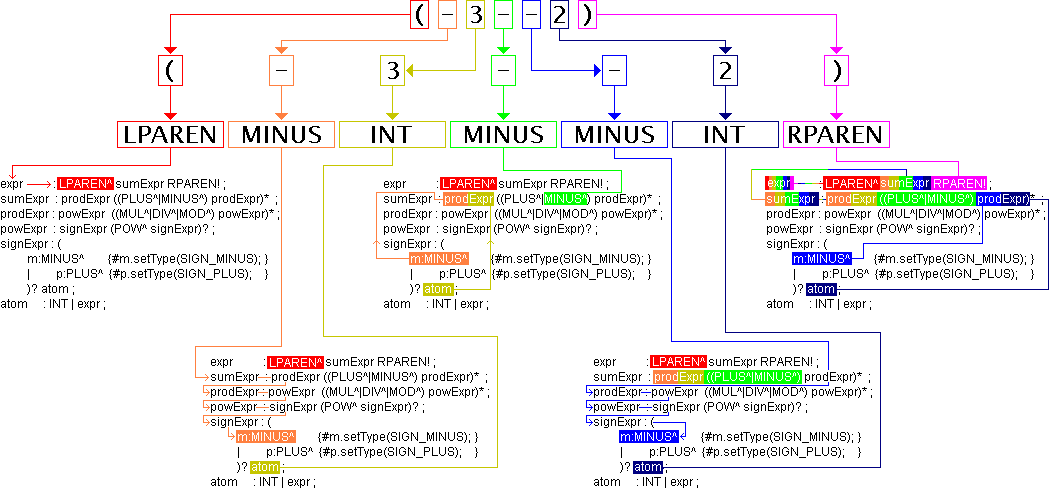
\includegraphics[scale=0.3]{sillyastthing}
  \end{center}
\end{frame}

\begin{frame}
  \frametitle{Lookahead parsing}
  \textbf{Lookahead} establishes the maximum incoming tokens that a parser can
  use to decide which rule it should use.  It is often explicitly indicated by
  affixing the lookahead to the algorithm name in parentheses, such as LALR(1)

  \vfill

Lookahead has two advantages:
\begin{itemize}
  \item It helps the parser take the correct action in case of
    \textbf{conflicts}. For example, parsing the \texttt{if} statement in the
    case of an \texttt{else} clause.

  \item It eliminates many duplicate states and eases the burden of an extra
    stack. A C language non-lookahead parser will have around 10,000 states. A
    lookahead parser will have around 300 states.
\end{itemize}
\end{frame}

\begin{frame}[fragile]
  \frametitle{Lookahead parsing: examples}
  Parsing the Expression 1 + 2 * 3.
  \vfill
\begin{verbatim}
Grammar is as follows:
 Rule1:  E -> E + E
 Rule2:  E -> E * E
 Rule3:  E -> number
 Rule4:  + has less precedence than *
\end{verbatim}
  \vfill
  \begin{center}
    %FIXME
    %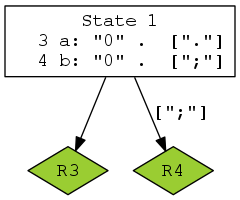
\includegraphics[scale=0.4]{example-reduce}
  \end{center}
\end{frame}

\begin{frame}
  \frametitle{LALR}
  In 1965, Donald Knuth invented the \textbf{LR} parser, which can recognize any
  deterministic context-free language in linear-bounded time. However, rightmost
  derivation has \textbf{very large memory requirements}

  \vfill

  In 1969, Frank DeRemer proposed a simplified version of the LR parser, namely
  the \textbf{Look-Ahead LR} (LALR). The simplification that takes place results
  in a parser with significantly reduced memory requirements but decreased
  language-recognition power. These parsers are seldom written by hand.
\end{frame}

\subsection{Shift/Reduce automaton}

\subsection{Formal grammars}


\begin{frame}
  \frametitle{Dangling else problem}
    \begin{itemize}[<+->]
      \item if a then if b then c else d
      \item To whom does the else belong?
      \item Shift/reduce conflict
    \end{itemize}
\end{frame}

\begin{frame}[fragile]
  \frametitle{Dangling else problem}
\begin{verbatim}
    stmt:
      condition
    | exp

    condition:
      "if" exp "then" stmt
    | "if" exp "then" stmt "else" stmt
\end{verbatim}
\end{frame}

\begin{frame}
  \frametitle{Dangling else problem}
    \begin{itemize}[<+->]
      \item Precedence solution
      \item \texttt{\%precedence "then"}
      \item \texttt{\%precedence "else"}
    \end{itemize}
\end{frame}

\begin{frame}
  \frametitle{Dangling else problem}
    \begin{itemize}[<+->]
      \item Associativity solution
      \item \texttt{\%right "then" "else"}
    \end{itemize}
\end{frame}

\begin{frame}
  \frametitle{Dangling else problem}
    \begin{itemize}[<+->]
      \item Changing the language
      \item if a then if b then c fi else d fi
      \item Often not acceptable
    \end{itemize}
\end{frame}

\section{Getting started}

\begin{frame}
  \frametitle{Getting started}
    \begin{itemize}[<+->]
      \item Prologue
      \item Grammar
      \item Epilogue
    \end{itemize}
\end{frame}

\begin{frame}
  \frametitle{Prologue}
    \begin{itemize}[<+->]
      \item Declarations
      \begin{itemize}[<+->]
        \item \texttt{\%defines}
        \item \texttt{\%expect 0}
        \item \texttt{\%skeleton "lalr1.cc"}
      \end{itemize}
      \item Includes
      \begin{itemize}[<+->]
        \item C code at the top of the parser
      \end{itemize}
      \item Token list
      \begin{itemize}[<+->]
        \item Token list
        \item \texttt{\#define}
        \item Prototypes (yylex)
      \end{itemize}
  \end{itemize}
\end{frame}

\begin{frame}
  \frametitle{Grammar}
    \begin{itemize}[<+->]
      \item Rules
      \item Actions
    \end{itemize}
\end{frame}

\begin{frame}
  \frametitle{Grammar Rules}
    \begin{itemize}[<+->]
      \item Similar to BNF
      \item No compact way to describe optional elements/lists
      \item Beware of the \%empty!
    \end{itemize}
\end{frame}

\begin{frame}
  \frametitle{Grammar Actions}
    \begin{itemize}[<+->]
      \item C/C++ code run when the rule is recognized
      \item Create an AST, compute the result of an expression\ldots
      \item Usually at the end
      \item Can be mid-rule actions (lexer context change, \ldots)
    \end{itemize}
\end{frame}


\begin{frame}
  \frametitle{Epilogue}
    \begin{itemize}[<+->]
      \item Raw C/C++ code included at the end of the parser
      \item main() to make it a stand-alone parser
    \end{itemize}
\end{frame}

\section{GNU Bison internals}

\subsection{GNU M4}

\begin{frame}
\end{frame}

\section{Working with GNU}

\begin{frame}
  \frametitle{Contributing}
    \begin{itemize}[<+->]
      \item Open source
      \item Peer review (quality standards)
      \item Testsuite
      \item Patches (e-mail)
    \end{itemize}
\end{frame}

\begin{frame}
  \frametitle{Coding style}
    \begin{itemize}[<+->]
      \item GNU prototyping convention
      \item Recently switched from ansi C89 to C99
      \item Indentation
      \item Comments (nice format)
      \item Clean code
    \end{itemize}
\end{frame}

\begin{frame}
  \frametitle{Git}
    \begin{itemize}[<+->]
      \item Commit early, commit often
      \item Every commit passes the testsuite (and compiles, of course!)
      \item A bugfix comes with a test
      \item Patch, integrated by the maintainers (Akim)
      \item String commit formatting
    \end{itemize}
\end{frame}

\begin{frame}
  \frametitle{Testsuite}
    \begin{itemize}[<+->]
      \item m4 macros
      \item Not unit-tests
      \item TESTSUITEFLAGS (specific tests, threading, \ldots)
      \item Testsuite needs to be compiled
    \end{itemize}
\end{frame}

\end{document}
